\section{Refining Intuitions through Practice}
\label{act1.1.6}

\begin{overview}

	\noindent
	{\bfseries Overview:} Remember how we \hyperref[ReadingRefiningIntuitions]{talked about ``refining intuitions''} and becoming so familiar with using our models that they become ``second nature'' to us? For that to happen, we need to practice using our models even more. This is what the following activities are all about. We'll attempt to make sense of more thermal phenomena by using the \ThreePhaseModel{} and the \EnergyInteractionModel{}, so that we'll become able to intuitively use them in new situations.
	
\end{overview}



\subsection{Energy in ice and liquid water}

\note{Timing: \unit[\textless5]{min}}{
	\subsubsection*{Principal learning goal}
	To learn to use the model to develop an answer that may not be immediately obvious by translating the process or situation in question into the ``language'' of the model, often in the form of a diagram, and then searching for implications or inconsistencies based on the logic of the model.
}

\begin{fnt}
	\label{fnt1.1.3-4}

Use the \EnergyInteractionModel{} to explain whether the following statement is true or false.

\todo[inline]{Seems like the \textdegree C unit was not converted to using the \texttt{\textbackslash unit} command. I've changed this below, but it should be globally changed somehow if it's not changed in general...

-BH}
\todo[inline]{I think the spacing in the italics didn't play well with the \textdegree C unit. It shouldn't need fixing anywhere else unless there are other instances of \textdegree C in italics. Using the \texttt{\textbackslash unit} command puts too much space between the number and the unit when we're doing degrees, in my opinion.

-EH}
\todo[inline]{Alright, I changed it from being in italics to being in quotes. Looks better that way. I do like the spacing between the number and the degree sign... Could you add this to the python script? I looked at it but can't really make sense of it, so I'd rather not mess with it...

-BH}

\begin{quote}
	``A quantity of ice at \unit[0]{\textdegree C} must contain less total energy than the same quantity of water at \unit[0]{\textdegree C}.''
\end{quote}
\end{fnt}

\noindent Make an \EnergyDiagram{} that relates the initial and final states described in the FNT. Use the diagram, and the logic of the model to explain which state would have more total energy.

\note{Answer to question}{
	By using an \EnergyDiagram{}, it should be obvious that energy had to be added to the ice to break some bonds (bond energy went up), while the thermal energy is unchanged (according to the simple version of our model, which we extend when we develop a particle model of bond and thermal energy), so the liquid water has more energy.
}
\note{FYI}{
	There is often a change of thermal energy at a phase change, due to a change in the heat capacity, but we are ignoring this for now in our simple model.  Don't bring this up with the students yet.  Everyone will eventually be able to deal with several subtle aspects like this, but not until we have mastered some basic thermodynamic relationships.
}

\WCD
\note{}{
	Have one or two groups give a careful explanation using the logic of the model.  Every statement must come from the model or be justified in some way (logic of the model).  Students are not used to doing this.  Emphasize it.  This is often where students falter on quizzes.
}

\subsection{The physical concept of \emph{Heat}}

\note{Timing: \unit[\about1]{min}}{
	\subsubsection*{Purpose}
	
	To emphasize the importance of knowing and using correct definitions of technical terms. In this case, the technical term is ``heat'' and how it is now used in both chemistry and physics texts, in contrast to how it was used historically.
}

\begin{fnt}
	\label{fnt1.1.3-5}

 According to the definition of heat in your course notes (pages 8 \& 16), can an energy system contain a certain amount of heat? Explain.
\end{fnt}

\noindent Discuss your response for this FNT with your group mates. Make sure everyone in your group is prepared to explain to the whole class. This is a group responsibility!

\note{Optimal response}{
	The important point is that ``heat'' has a technical definition that is much more restricted than its use in everyday English. Heat is a {\em transfer} of energy between two physical things as a result of a temperature difference between them.
}

\WCD
\note{}{
	Give them a couple of minutes to discuss in their Small Groups (SG), and have someone explain to the Whole Class.  You should comment that historically, the word ``heat'' was often used for what we now call thermal energy.  Some older textbooks will use ``heat'' this way.  This is one of those cases where you need to read critically, to know how a word is being used.  All newer introductory textbooks in both chemistry and physics we are aware of, however, use the term ``heat'' as we have defined it here.
}

\subsection{Equilibrating Copper and Water}

\note{Timing: \unit[\about20]{min} total for all parts, not including WC discussions}{
	Notice that there are two WC discussions, one after they put parts 1 and 2 on the board, and then one after they respond to part 3.
}

\begin{fnt}
	\label{fnt1.1.3-6}

Imagine that you place a piece of copper with an initial temperature of \unit[20]{\textdegree C} in contact with an amount of liquid water with an initial temperature of \unit[100]{\textdegree C}. Assume that the physical system consisting of the copper and the water is thermally isolated from everything else; i.e., water and copper can \emph{only} exchange energy \emph{with each other}.

\begin{enumerate}[(a)]
	\item Using the \ThreePhaseModel{} as applied to each substance and your understanding of what ``coming to thermal equilibrium'' means:
	
	\begin{enumerate}[i.]
		\item Sketch two \TempGraphs{} -- one for each substance -- and indicate the initial state for each one.
		\item Explain in a sentence or two how you can tell if either substance will undergo a phase change during the process of coming to thermal equilibrium. You are expected to use what you already know regarding the thermal properties of copper and water, but you do not need to do any calculations.
	\end{enumerate}
	
	\item Construct a complete \EnergyDiagram{} for the process that ends when the two substances are in thermal equilibrium. Don't forget that a complete diagram always includes an algebraic expression of energy conservation.
	
	\item Now consider a similar process. Use the same initial conditions for the copper, but assume that the \ce{H2O} is initially in the gas phase at \unit[100]{\textdegree C}.
	\begin{enumerate}[i.]
		\item Sketch two \TempGraphs{}, one for each substance, and mark the initial state for each one.
		\item How can you determine if the \ce{H2O} will undergo a temperature change? (What calculations and comparisons -- think energy -- would you need to make?  Don't actually do the calculations; just explain what you would need to do.)
	\end{enumerate}
\end{enumerate}
\end{fnt}

\begin{enumerate}
	\item Put your \TempGraphs{} on the board with the initial state marked on each one. Explain briefly how you can tell if either substance might undergo a phase change during this process.
	
	\note{For example}{
		``Given the initial states on a \TempGraph{}, neither substance will reach a phase change temperature as energy in the form of heat is transferred between them'', or, ``There are no phase change temperatures for either substance in the range of possible final temperatures.''
	}

	\item Put your complete \EnergyDiagram{} on the board for this process.
	
	If ${\Delta E_\text{thermal(Cu)} = \text{\unit[250]{kJ}}}$, what is $\Delta E_{\text{thermal}\left(\text{H}_2\text{O}\right)}$? Explain why.
	
	\note{}{
		\noindent
		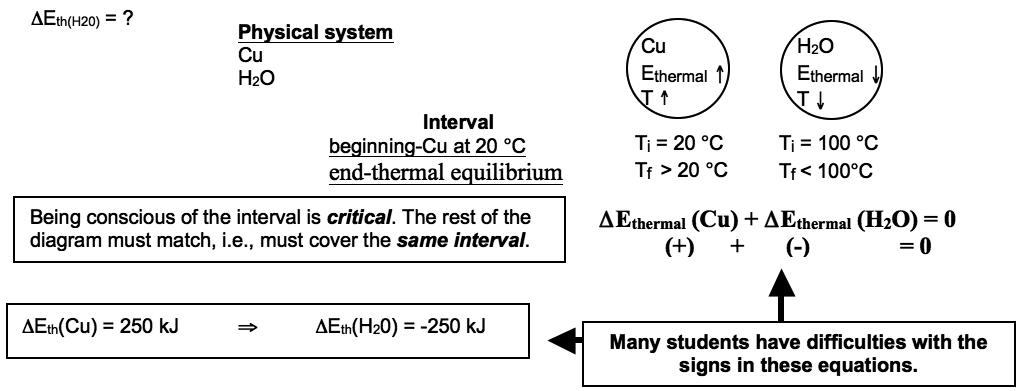
\includegraphics[width=\linewidth]{act116-b}
	}
	
\WCD

	\note{}{
		Do any clarifying that is necessary, but try to get the students to do most of the explaining. 
		
		At the end of this whole-class discussion, ask the question: ``Why was it necessary to ask part (b) after part (a) and not vice-versa?''
		
		Answer: To apply the \EnergyInteractionModel{} you have to know what energy systems are involved.  In this particular case, that means knowing whether or not there will be a phase change of either of the substances.  
	}
	
	\item Redraw your \TempGraphs{} for the new initial conditions. Explain briefly how you could determine if the \ce{H2O} will undergo a phase change or temperature change.
	
	\note{The students will need to be able to do this kind of analysis in DLM03!}{
		\todo[inline]{What is this reference to DLM03 in DLM4 using future tense about?}
		Help them figure out that they need to compare the magnitude of energy needed to increase the temperature of the Cu to 100$^\circ$C with the magnitude of energy lost by the \ce{H2O} as it completes its phase change to decide if the \ce{H2O} will change temperature.
		\begin{itemize}
			\item If the former is smaller, when the Cu reaches 100$^\circ$C the \ce{H2O} will only be partway through its phase change, and the process will stop (thermal equilibrium). 
			\item If the former is larger, the \ce{H2O} will complete its phase change before the Cu reaches 100$^\circ$, and the process will continue until thermal equilibrium is reached. 
		\end{itemize}
	}
\end{enumerate}

\WCD

\note{}{
	Try to get the students to do most of the explaining, but make sure all of the important points are covered.
}